\documentclass{sigchi}

% Use this command to override the default ACM copyright statement
% (e.g. for preprints).  Consult the conference website for the
% camera-ready copyright statement.

%------------------------- COPYRIGHT ---------------------------------------------
\toappear{Permission to make digital or hard copies of all or part of this work for personal or classroom use is granted without fee provided that copies are not made or distributed for profit or commercial advantage and that copies bear this notice and the full citation on the first page. Copyrights for components of this work owned by others than ACM must be honored. Abstracting with credit is permitted. To copy otherwise, or republish, to post on servers or to redistribute to lists, requires prior specific permission and/or a fee. Request permissions from permissions@acm.org. \\
{\emph{TEI '16}}, February 14-17, 2016, Eindhoven, Netherlands. \\
Copyright \copyright~2016 ACM ISBN/978-1-4503-3582-9/16/02\$15.00. \\
DOI http://dx.doi.org/10.1145/2839462.2854103
 }

% Arabic page numbers for submission.  Remove this line to eliminate
% page numbers for the camera ready copy
%\pagenumbering{arabic}

% Load basic packages
\usepackage{balance}  
\usepackage{graphics} 
\usepackage[T1]{fontenc}
\usepackage{txfonts}
\usepackage{mathptmx}
\usepackage[pdftex]{hyperref}
\usepackage{color}
\usepackage{booktabs}
\usepackage{textcomp}
\usepackage{microtype} 
\usepackage[all]{hypcap}  
\usepackage{ccicons}
\usepackage[labelsep=period]{caption}
\usepackage[labelsep=period]{subcaption}
\usepackage[inline]{enumitem}
\usepackage{fixltx2e}
\usepackage[super]{nth}

% Shortcut to typeset table headings
\newcommand\tabhead[1]{\small\textbf{#1}}

% llt: Define a global style for URLs
\makeatletter
\def\url@leostyle{%
  \@ifundefined{selectfont}{
    \def\UrlFont{\sf}
  }{
    \def\UrlFont{\small\bf\ttfamily}
  }}
\makeatother
\urlstyle{leo}

% Page size
\def\pprw{8.5in}
\def\pprh{11in}
\special{papersize=\pprw,\pprh}
\setlength{\paperwidth}{\pprw}
\setlength{\paperheight}{\pprh}
\setlength{\pdfpagewidth}{\pprw}
\setlength{\pdfpageheight}{\pprh}

%------------------------- METADATA ---------------------------------------------
\def\plaintitle{Embodied Spatial Thinking in Tangible Computing}
\def\plainauthor{Brendan Alexander Harmon}
\def\emptyauthor{} % for submitting for anonymous review
\def\plainkeywords{Human-computer interaction; tangible user interfaces; 
tangible interaction; embodied cognition; spatial thinking; 3D modeling} % creativity
\def\plaingeneralterms{Design}

\definecolor{linkColor}{RGB}{6,125,233}
\hypersetup{%
  pdftitle={\plaintitle},
% Use \plainauthor for final version.
%  pdfauthor={\plainauthor},
  pdfauthor={\emptyauthor},
  pdfkeywords={\plainkeywords},
  bookmarksnumbered,
  pdfstartview={FitH},
  colorlinks,
  citecolor=black,
  filecolor=black,
  linkcolor=black,
  urlcolor=linkColor,
  breaklinks=true,
}

%------------------------- DOCUMENT ---------------------------------------------

\begin{document}

\title{Embodied Spatial Thinking in Tangible Computing}

\numberofauthors{1}
\author{%
  \alignauthor{Brendan Alexander Harmon\\
    \affaddr{North Carolina State University}\\
    \affaddr{Raleigh, USA}\\
    \email{brendan.harmon@gmail.com}}\\
}

\maketitle

%------------------------- ABSTRACT ---------------------------------------------

\begin{abstract} % 150 words
%The abstract should be a concise statement of the problem, approach, and
% conclusions of the work described. It should clearly state the paper's
% contribution to the field of HCI

Tangible user interfaces are based on the premise
that embodied cognition in computing
can enhance cognitive processes.
%
However, the ways in which embodied cognition in computing
transform spatial thinking have not yet been rigorously studied.
%
I have co-designed Tangible Landscape --
a continuous shape display 
powered by a geographic information system --
and used it to explore how 
technology mediates spatial cognition %and creativity
in a rigorous experiment. 

% experiment
In this terrain modeling experiment 
I use geospatial analytics 
%such as geomorphometry and geostatistics
% supplemented by semi-structured interviews and direct observation
to analyze how %quantitatively and qualitatively 
visual computing with a GUI
and tangible computing with a shape display
mediate multidimensional spatial performance. 

% findings
My initial findings suggest that: 
\begin{enumerate*}[label=\bfseries \arabic*.]
\item digital sculpting via a GUI 
is unintuitive, 
%and visual ambiguity and misreadings 
%lead to spatial misinterpretations,
\item shape displays like Tangible Landscape can be intuitive, 
enhance spatial performance, and
%in novel ways
enable rapid iteration and ideation,
%enable rapid iterations of generative form-finding and critical analysis, 
%and encourage creativity, 
and
\item different analytics encourage 
significantly different modes of spatial thinking 
and strategies for modeling. 
\end{enumerate*}

%% conclusions
%In conclusion 
%intuitive, kinaesthetic interaction 
%with useful computational analytics 
%can enhance spatial thinking.

\end{abstract}


\category{H.5.2.}{Information Interfaces and Presentation 
(e.g. HCI)}{User Interfaces -- Evaluation/methodology; Interaction styles; 
Prototyping; Theory and methods} 
%\category{H.5.m.}{Information Interfaces and Presentation (e.g. HCI)}{Miscellaneous} 
%See \url{http://acm.org/about/class/1998/} for the full list of ACM classifiers.

\keywords{\plainkeywords}

%------------------------- BRIEF ---------------------------------------------

%The paper should provide a research description covering central 
%aspects of the PhD work, describing the context and motivation, 
%the main research objectives and questions, a short background/
%literature review relevant to frame the research, a description and 
%rationale for research approach and methods, and a description of 
%selected results if applicable. Finally, the document should describe 
%an outline of the activities done so far and activities planned for the 
%remainder of the PhD. 

%------------------------- INTRO ---------------------------------------------

% Describe the context and motivation, 
% the main research objectives and questions, 
% and a short literature review relevant to frame the research.

\section{Introduction}

%% cognitive science
%There is a new paradigm of cognitive science that studies 
%`cognition beyond the brain' \cite{Hardy-Vallee2008}
%and has inspired new modes computing.
%This new paradigm -- embodied, situated, and distributed cognition -- 
%explores how cognition is functionally embedded in the body, 
%embedded in its environment, 
%and distributed across networks of agents and artifacts. 
%While older paradigms of cognitive science 
%studied the mind abstracted in isolation, 
%this paradigm grounds cognition in its biocultural context studying 
%how a continuous flow of information 
%links brain, body, and environment \cite{Hardy-Vallee2008}.
In embodied cognition
%an emerging paradigm of cognitive science
the mind is embedded in the body. 
%and based on bodily experience. 
Higher cognitive processes
% the traditional realm of cognitive science
rely on lower level processes
such as emotion and sensorimotor processes 
that link perception and action \cite{Hardy-Vallee2008}. 
Thus body and action mediate thought. 
Cognitive processes can be physically simulated 
with cognition offloaded onto action. %\cite{Kirsh2013}
Objects such as tools can be cognitively grasped and temporarily, 
contingently incorporated into ones body schema \cite{Kirsh2013}.
This view of cognition considers feeling, action, and perception 
to be functionally integral to thought.

% design theory and implementation
Based on the theory of embodied cognition
researchers have theorized a physical-digital divide in human-computer interaction --
positing that 
the high level of abstraction required to interact with a computer
via a graphical user interface (GUI) in a visual computing paradigm 
constrains how we think -- 
and designed innovative technologies for bridging this divide 
such as tangible user interfaces (TUIs) \cite{Ishii1997, Dourish2001}. 
%If ``GUIs fall short of embracing the richness of human senses and skills 
%people have developed through a lifetime of interaction with the physical world'' 
%then TUIs could
%``bridge the gaps between both cyberspace and the physical environment, 
%as well as the foreground and background of human activities'' \cite{Ishii1997}.
%
%In their vision of TUIs 
%digital data would be physically embodied as tangible bits 
%so that users could feel and not just see their data. 
%By physically manifesting digital data they hoped to offer new affordances -- 
%the ability to touch and sense the size, shape, volume, weight, texture, and hardness of the data; 
%the ability to directly, physically manipulate and shape data \cite{Ishii1997}. 
%
TUIs are designed to physically manifest digital data as tangible bits 
that afford the ability to directly, physically feel and manipulate data \cite{Ishii1997}. 
%
%To, in terms of cognitive neuroscience, make pragmatic representations of digital data. 
%Pragmatic representations are internal, conceptual models for rapidly generating action
%that are primarily based on tactile feedback,
%on direct assessments of the form and physical properties of objects.
%This tactile feedback is processed automatically, immediately, 
%and subconsciously \cite{Jeannerod1997}. 
%
TUIs make pragmatic representations of digital data. 
Pragmatic representations are conceptual models for rapidly generating action
that are primarily based on tactile feedback and are processed automatically, immediately, 
and subconsciously \cite{Jeannerod1997}. 
%
By physically manifesting data so that we can pragmatically
interact with computations,  
TUIs should enable rapid, intuitive action and expression 
in a way that was not possible in visual computing. 
By enabling embodied cognition in human-computer interaction 
TUIs should let us cognitively grip data as an extension of our bodies, 
intuitively manipulate data, and physically simulate processes. 
This should enhance spatial thinking.

%% spatial learning
%Spatial thinking is malleable and can be improved with training. 
%Spatial training has been shown to improve performance 
%in science, technology, engineering, and math (STEM) \cite{Uttal2013}. 
%More embodied spatial thinking may lead to improvements in 
%STEM performance by enhancing perception
%and reducing cognitive loads with 
%pragmatic representations and physical simulation. 
%Since spatial thinking is mediated by technology 
%the effectiveness of training methods will depend 
%upon their implementation, upon the technology used. 
%Unintuitive human-computer interaction may constrain spatial thinking 
%and add cognitive costs thus reducing the effectiveness 
%of digitally implemented training methods. 
%Embodied and computationally enriched cognition 
%may enhance spatial thinking in novel ways
%enabling and encouraging coupled creative and analytic thinking.

% tangible user interaction
Research on TUIs has been more focused on the 
design and development of the technology 
than empirically testing the use and effects of the technology.
Rasmussen et al.\ for example discuss 
the focus on the design and development of shape displays 
rather than empirical research about their use. 
\cite{Rasmussen2012}.
% research directions
Research on tangible interaction has focused on user experience 
and to a lesser degree user performance 
using methods such as
%direct observation, 
participant observation, 
semi-structured interviews,
video analysis,
and small-scale experiments. 
%with metrics like
%task time completion.
% creative spatial cognition
%The few studies have explored creative spatial cognition 
%in tangible interaction
%have used protocol analysis \cite{Kim2008}. 

% research aim
While the theory of embodied cognition
has inspired the design of novel technologies 
for human-computer interaction,
its applied principles need to be empirically tested, 
critiqued, and refined in order to improve interaction design.  
The aim of this research is to study how tangible computing 
mediates spatial thinking in order to 
improve interaction design, enhance spatial performance, 
and improve spatial education. 
%My goal is to develop, test, and refine an empirically grounded theory of
%how technology mediates spatial cognition 
%that can inform spatial education and human-computer interaction design. 

%\subsection*{Research questions}
%\begin{enumerate}
%\item How do shape displays mediate spatial and creative thinking?
%\item How successfully can parallel embodied and computationally enriched analytical processes be coordinated? 
%\item Can embodied and computationally enriched cognition enhance spatial thinking in novel ways 
%by blending generative and analytic thinking? 
%\item What computational analytics most effectively improve spatial performance?
%\end{enumerate}

\subsection*{Testable hypotheses}
I hypothesize that:
\begin{enumerate}
	\item limited feedback constrains spatial performance,
	\item misinterpretations of 3D space in visual computing reduce spatial performance, 
	\item computational analytics like differencing and flow simulations can enhance spatial performance,
	\item computationally enriched analytical thinking can be coordinated with embodied thinking,
	\item tangible computing that computationally enhances embodied spatial thinking can improve spatial performance, and 
	\item tangible computing can enable a rapid iterative process of exploratory, generative form-finding that can improve spatial performance.
	%\item in which computational analytics are blended with embodied spatial cognition 
	%giving rise to a new form a creative, spatial thinking.
	
\end{enumerate}


%------------------------- METHODOLOGY ---------------------------------------------

% Describe the rationale for research approach and methods

\section{Methdology}

\setlength{\belowcaptionskip}{-0.5em}
%
\begin{figure*}[h]
%
\captionsetup{singlelinecheck=off}
%
        \centering
        \begin{subfigure}[t]{0.165\textwidth}
                \includegraphics[width=\textwidth]{{figures/tl/tl_schema.pdf}}
                %\caption{A cycle of scanning and projection couples a physical and digital model}
                \caption{}
                \label{fig:schema}
        \end{subfigure}
        ~ %add desired spacing between images, e. g. ~, \quad, \qquad, \hfill etc.
        \begin{subfigure}[t]{0.25\textwidth}
                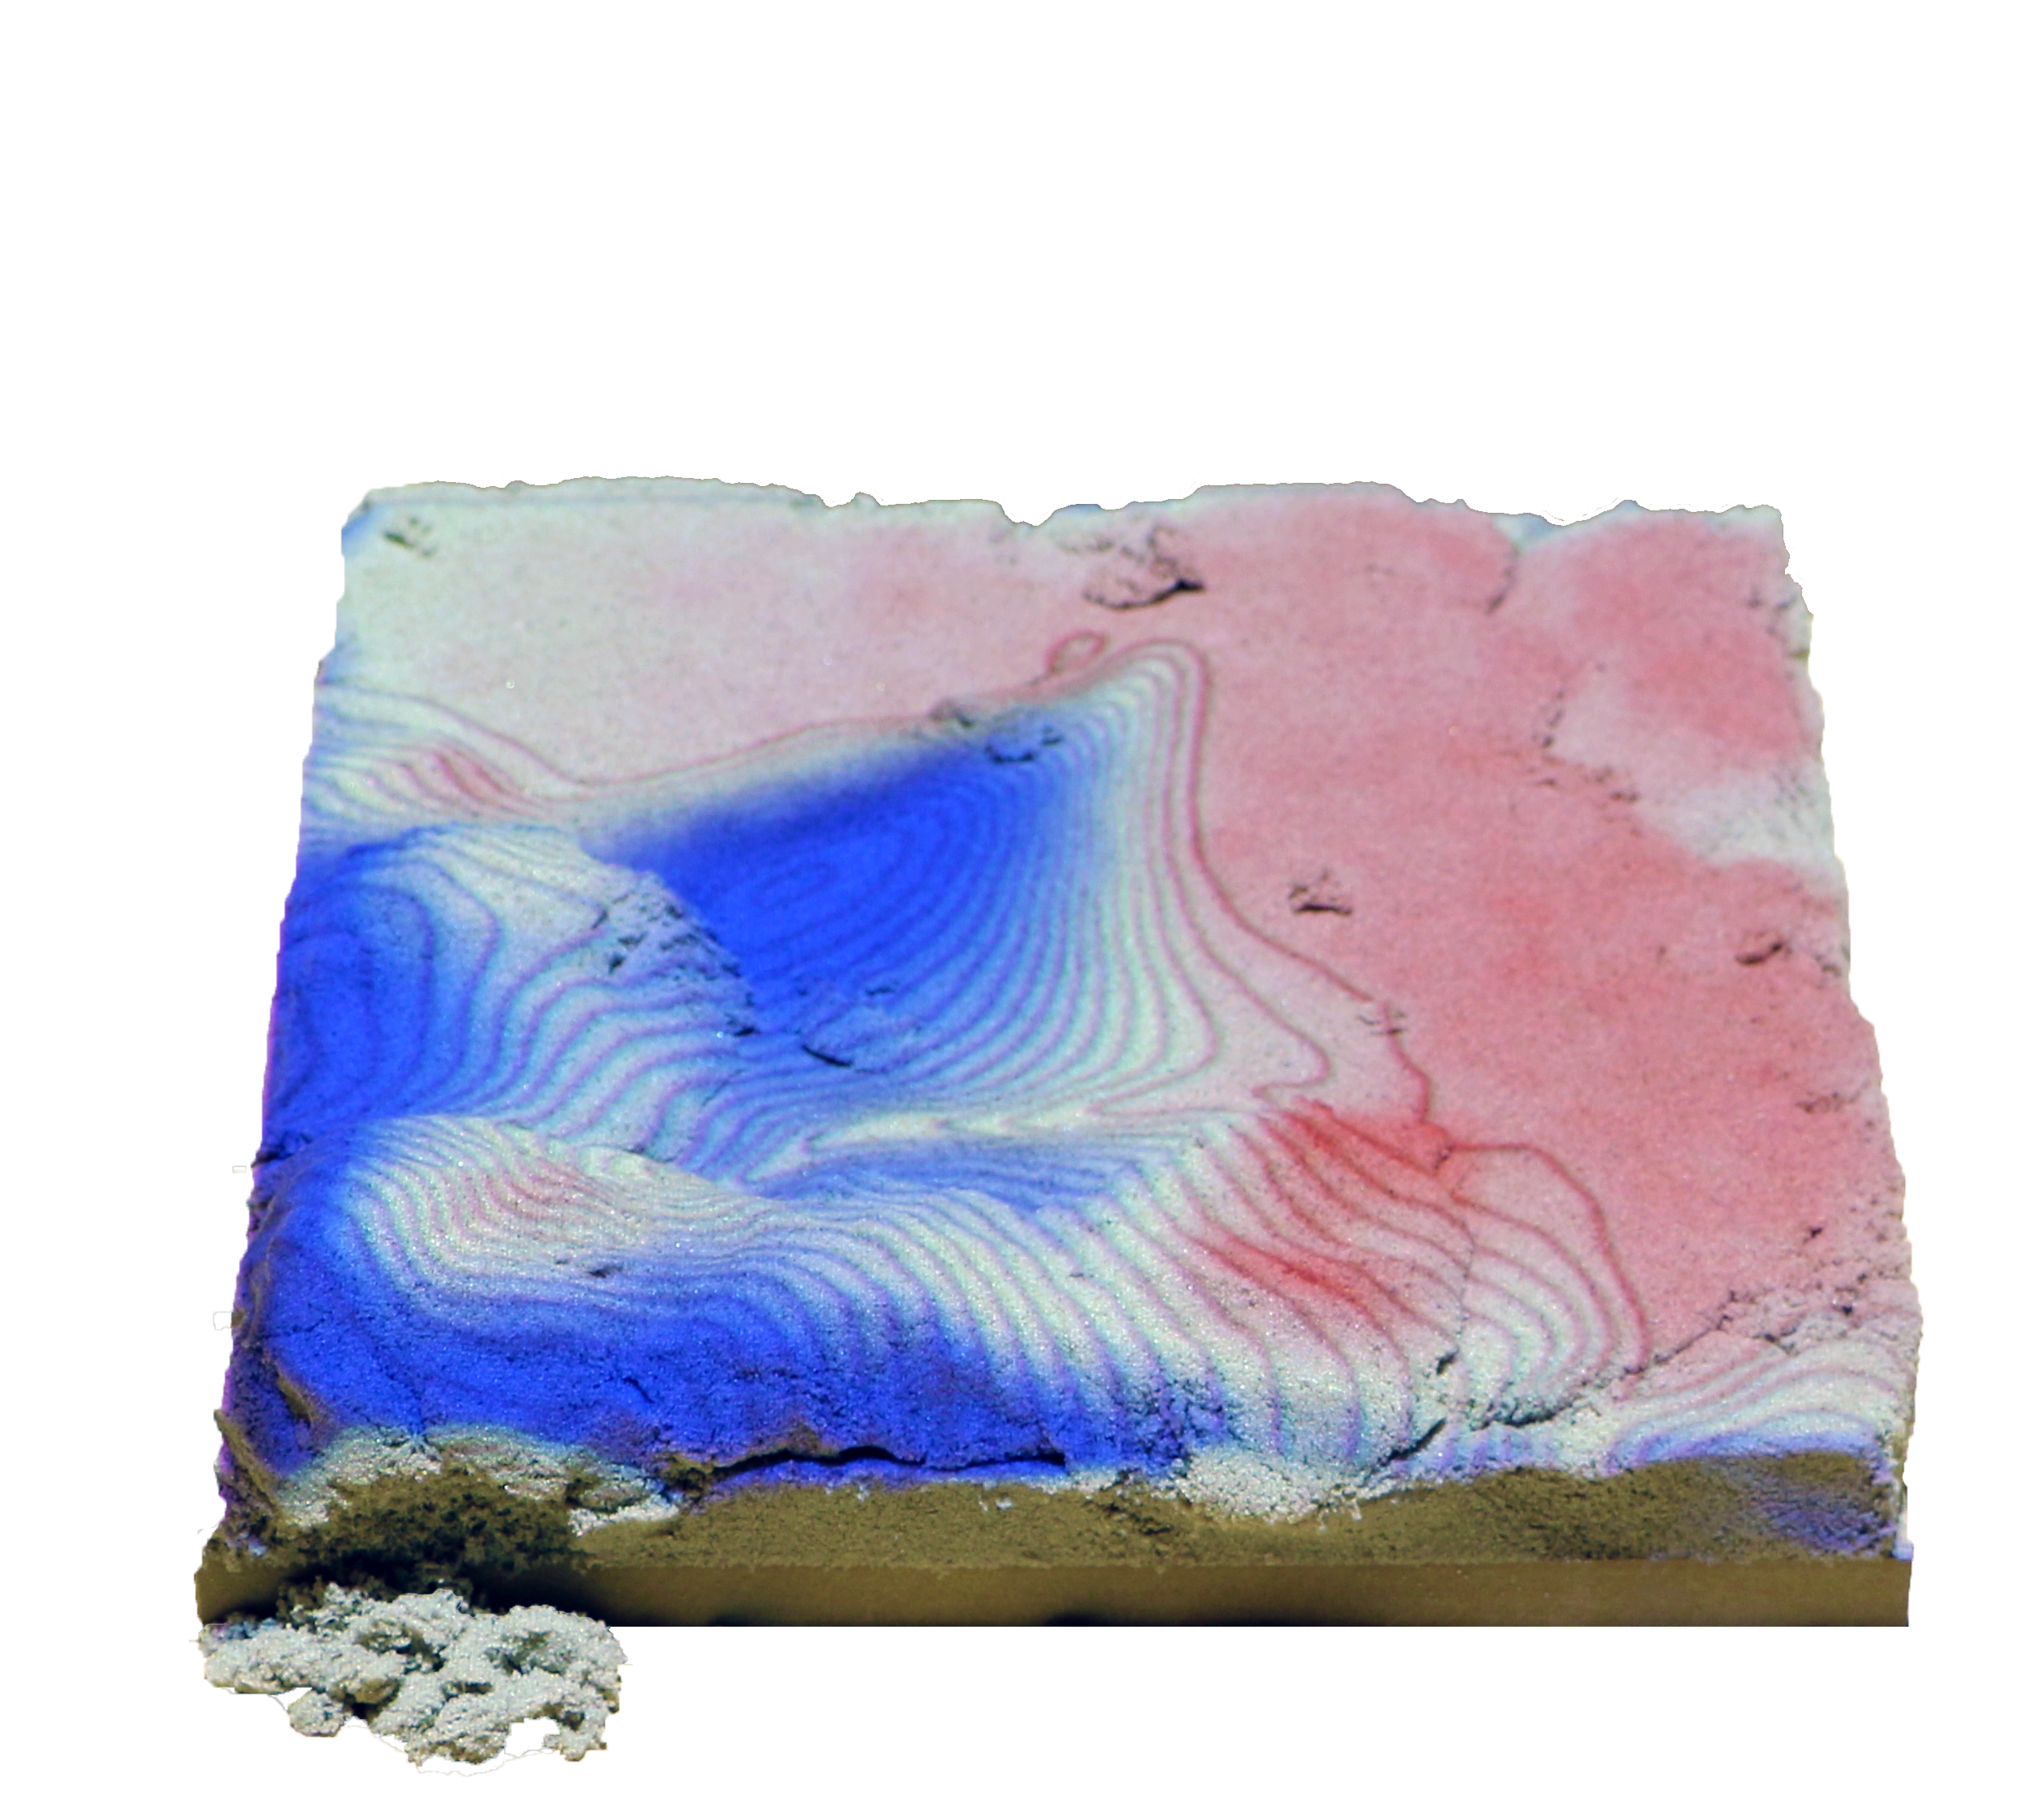
\includegraphics[width=\textwidth]{figures/tl/tl_difference_s_1.png}
                %\includegraphics[width=\textwidth]{images/art_diff_1}
                %\caption{Water flow}
                \caption{}
                \label{fig:sequence_0_2}
        \end{subfigure}
        ~ %add desired spacing between images, e. g. ~, \quad, \qquad, \hfill etc.
        \begin{subfigure}[t]{0.25\textwidth}
                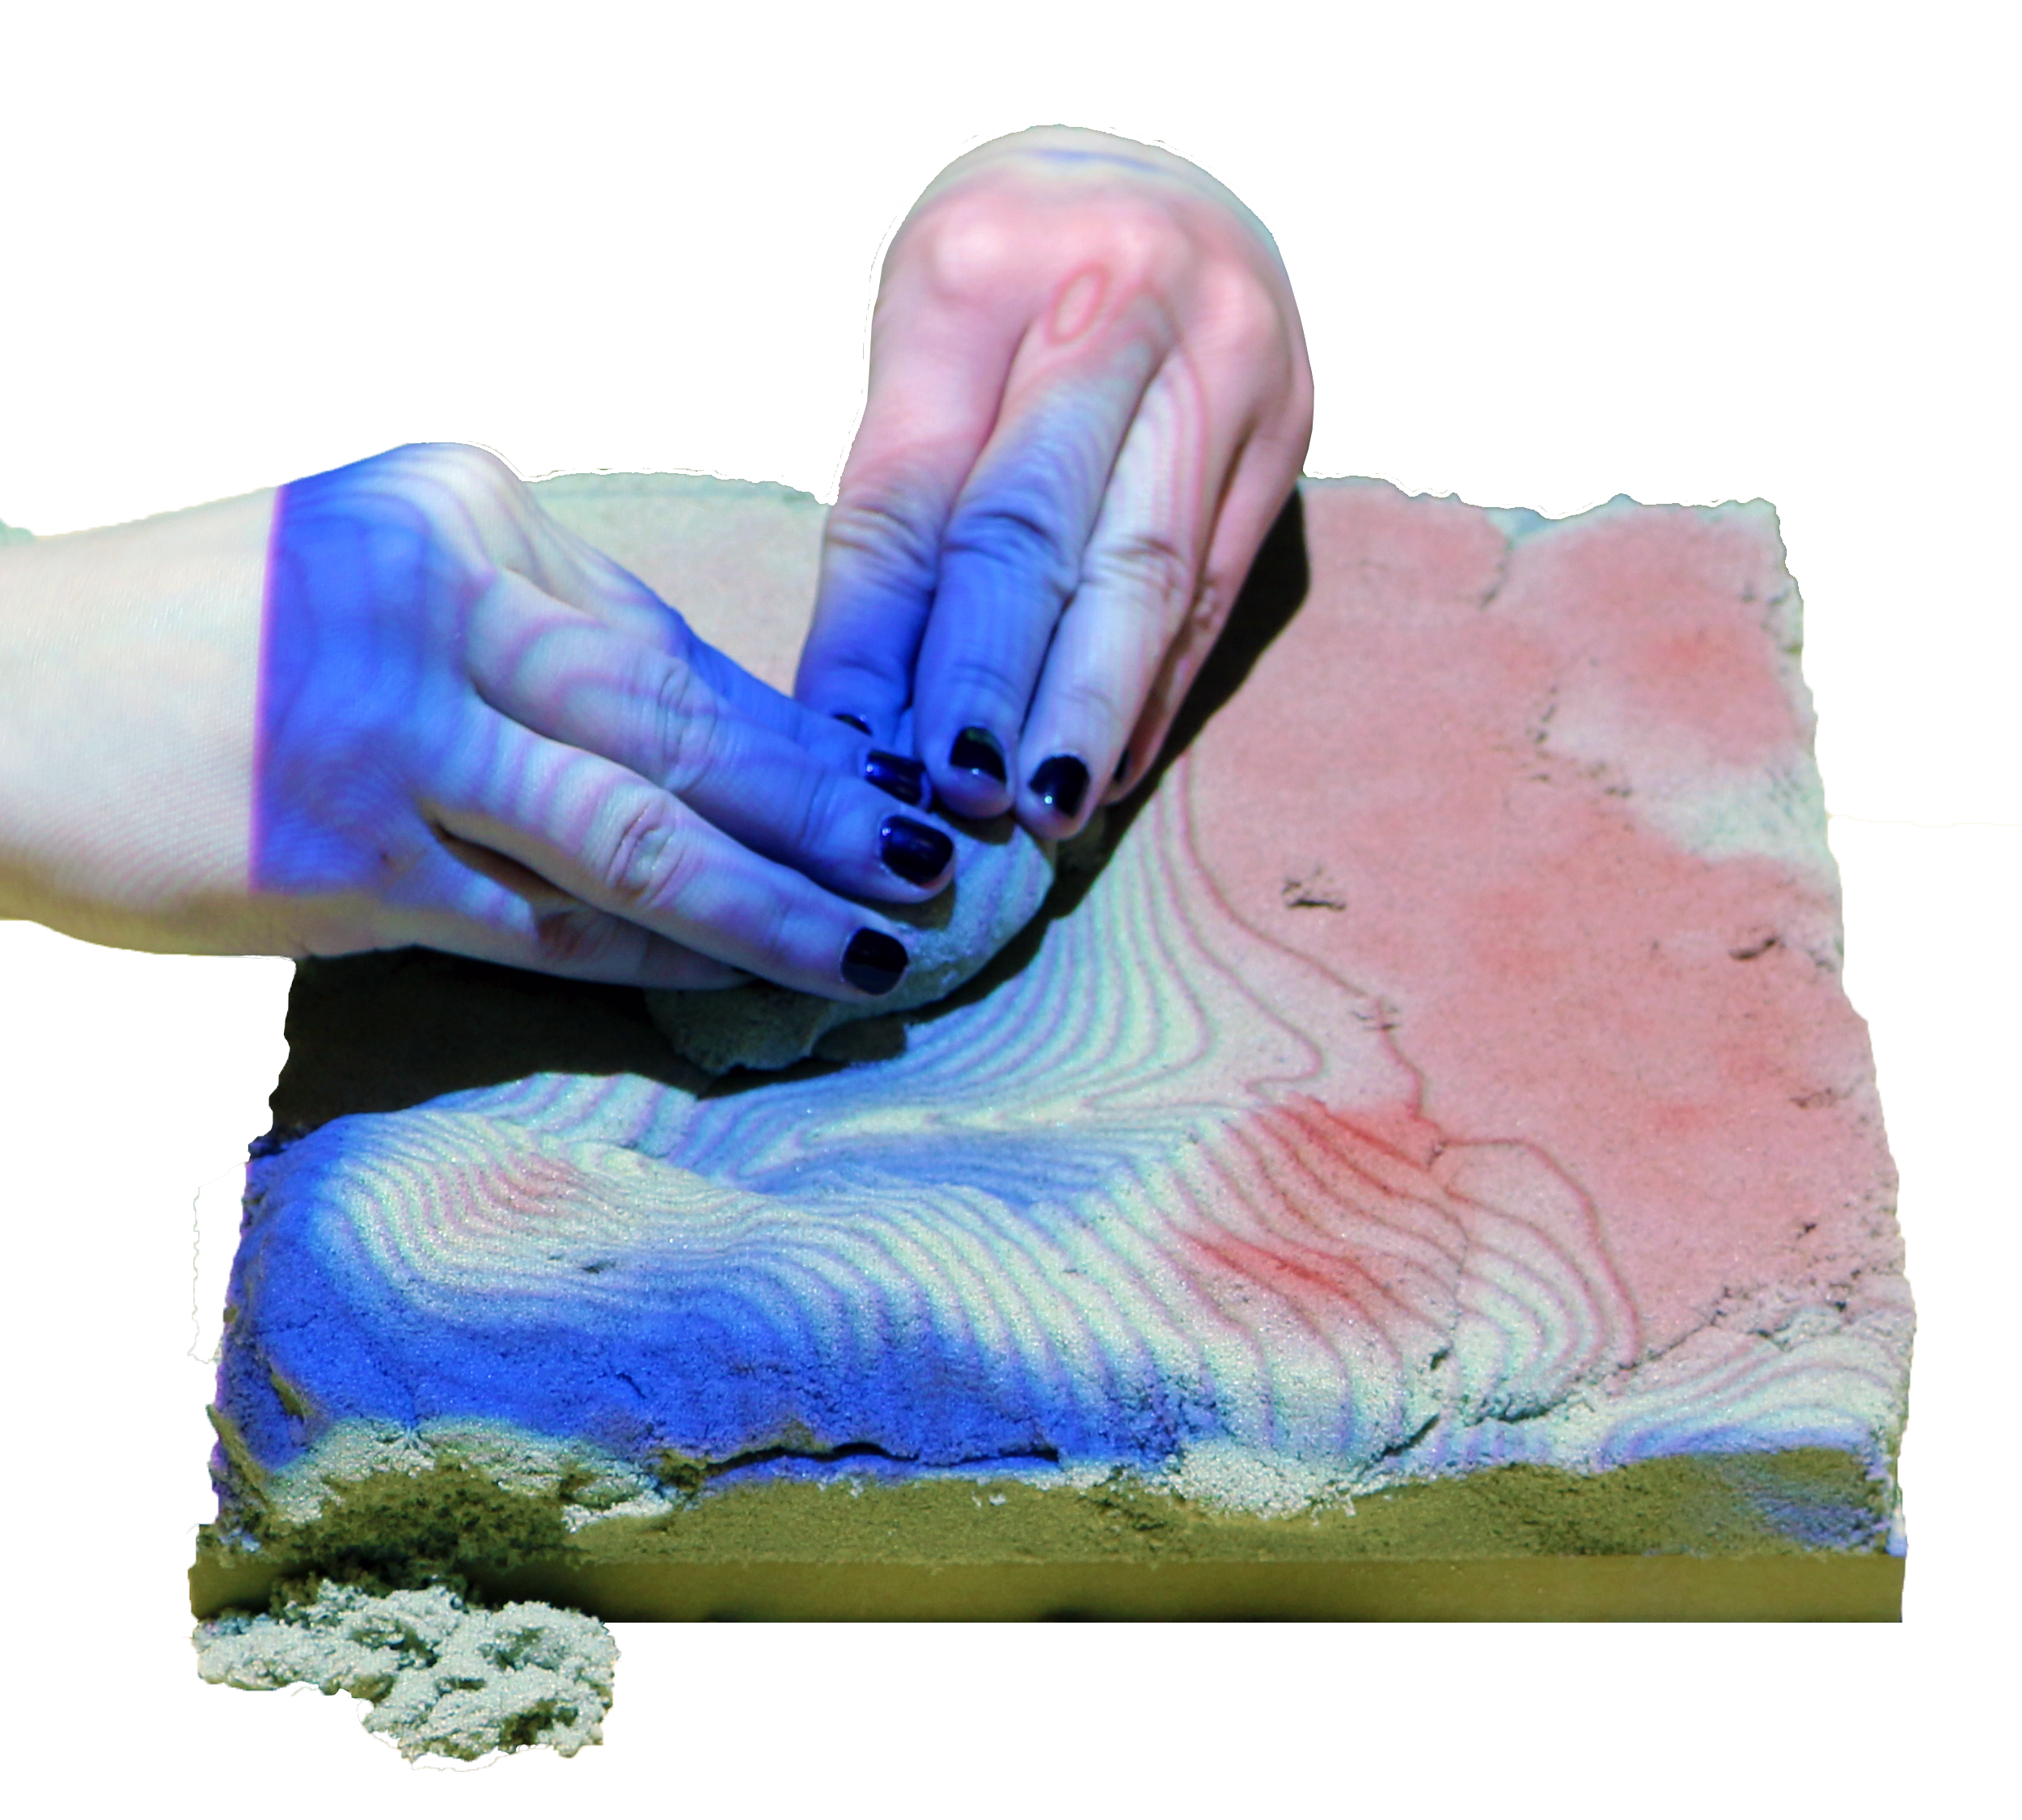
\includegraphics[width=\textwidth]{figures/tl/tl_difference_s_2.png}
                %\includegraphics[width=\textwidth]{images/art_diff_2}
                %\caption{Sculpting a check dam}
                \caption{}
                \label{fig:sequence_0_3}
        \end{subfigure}
        ~ %add desired spacing between images, e. g. ~, \quad, \qquad, \hfill etc.
        \begin{subfigure}[t]{0.25\textwidth}
                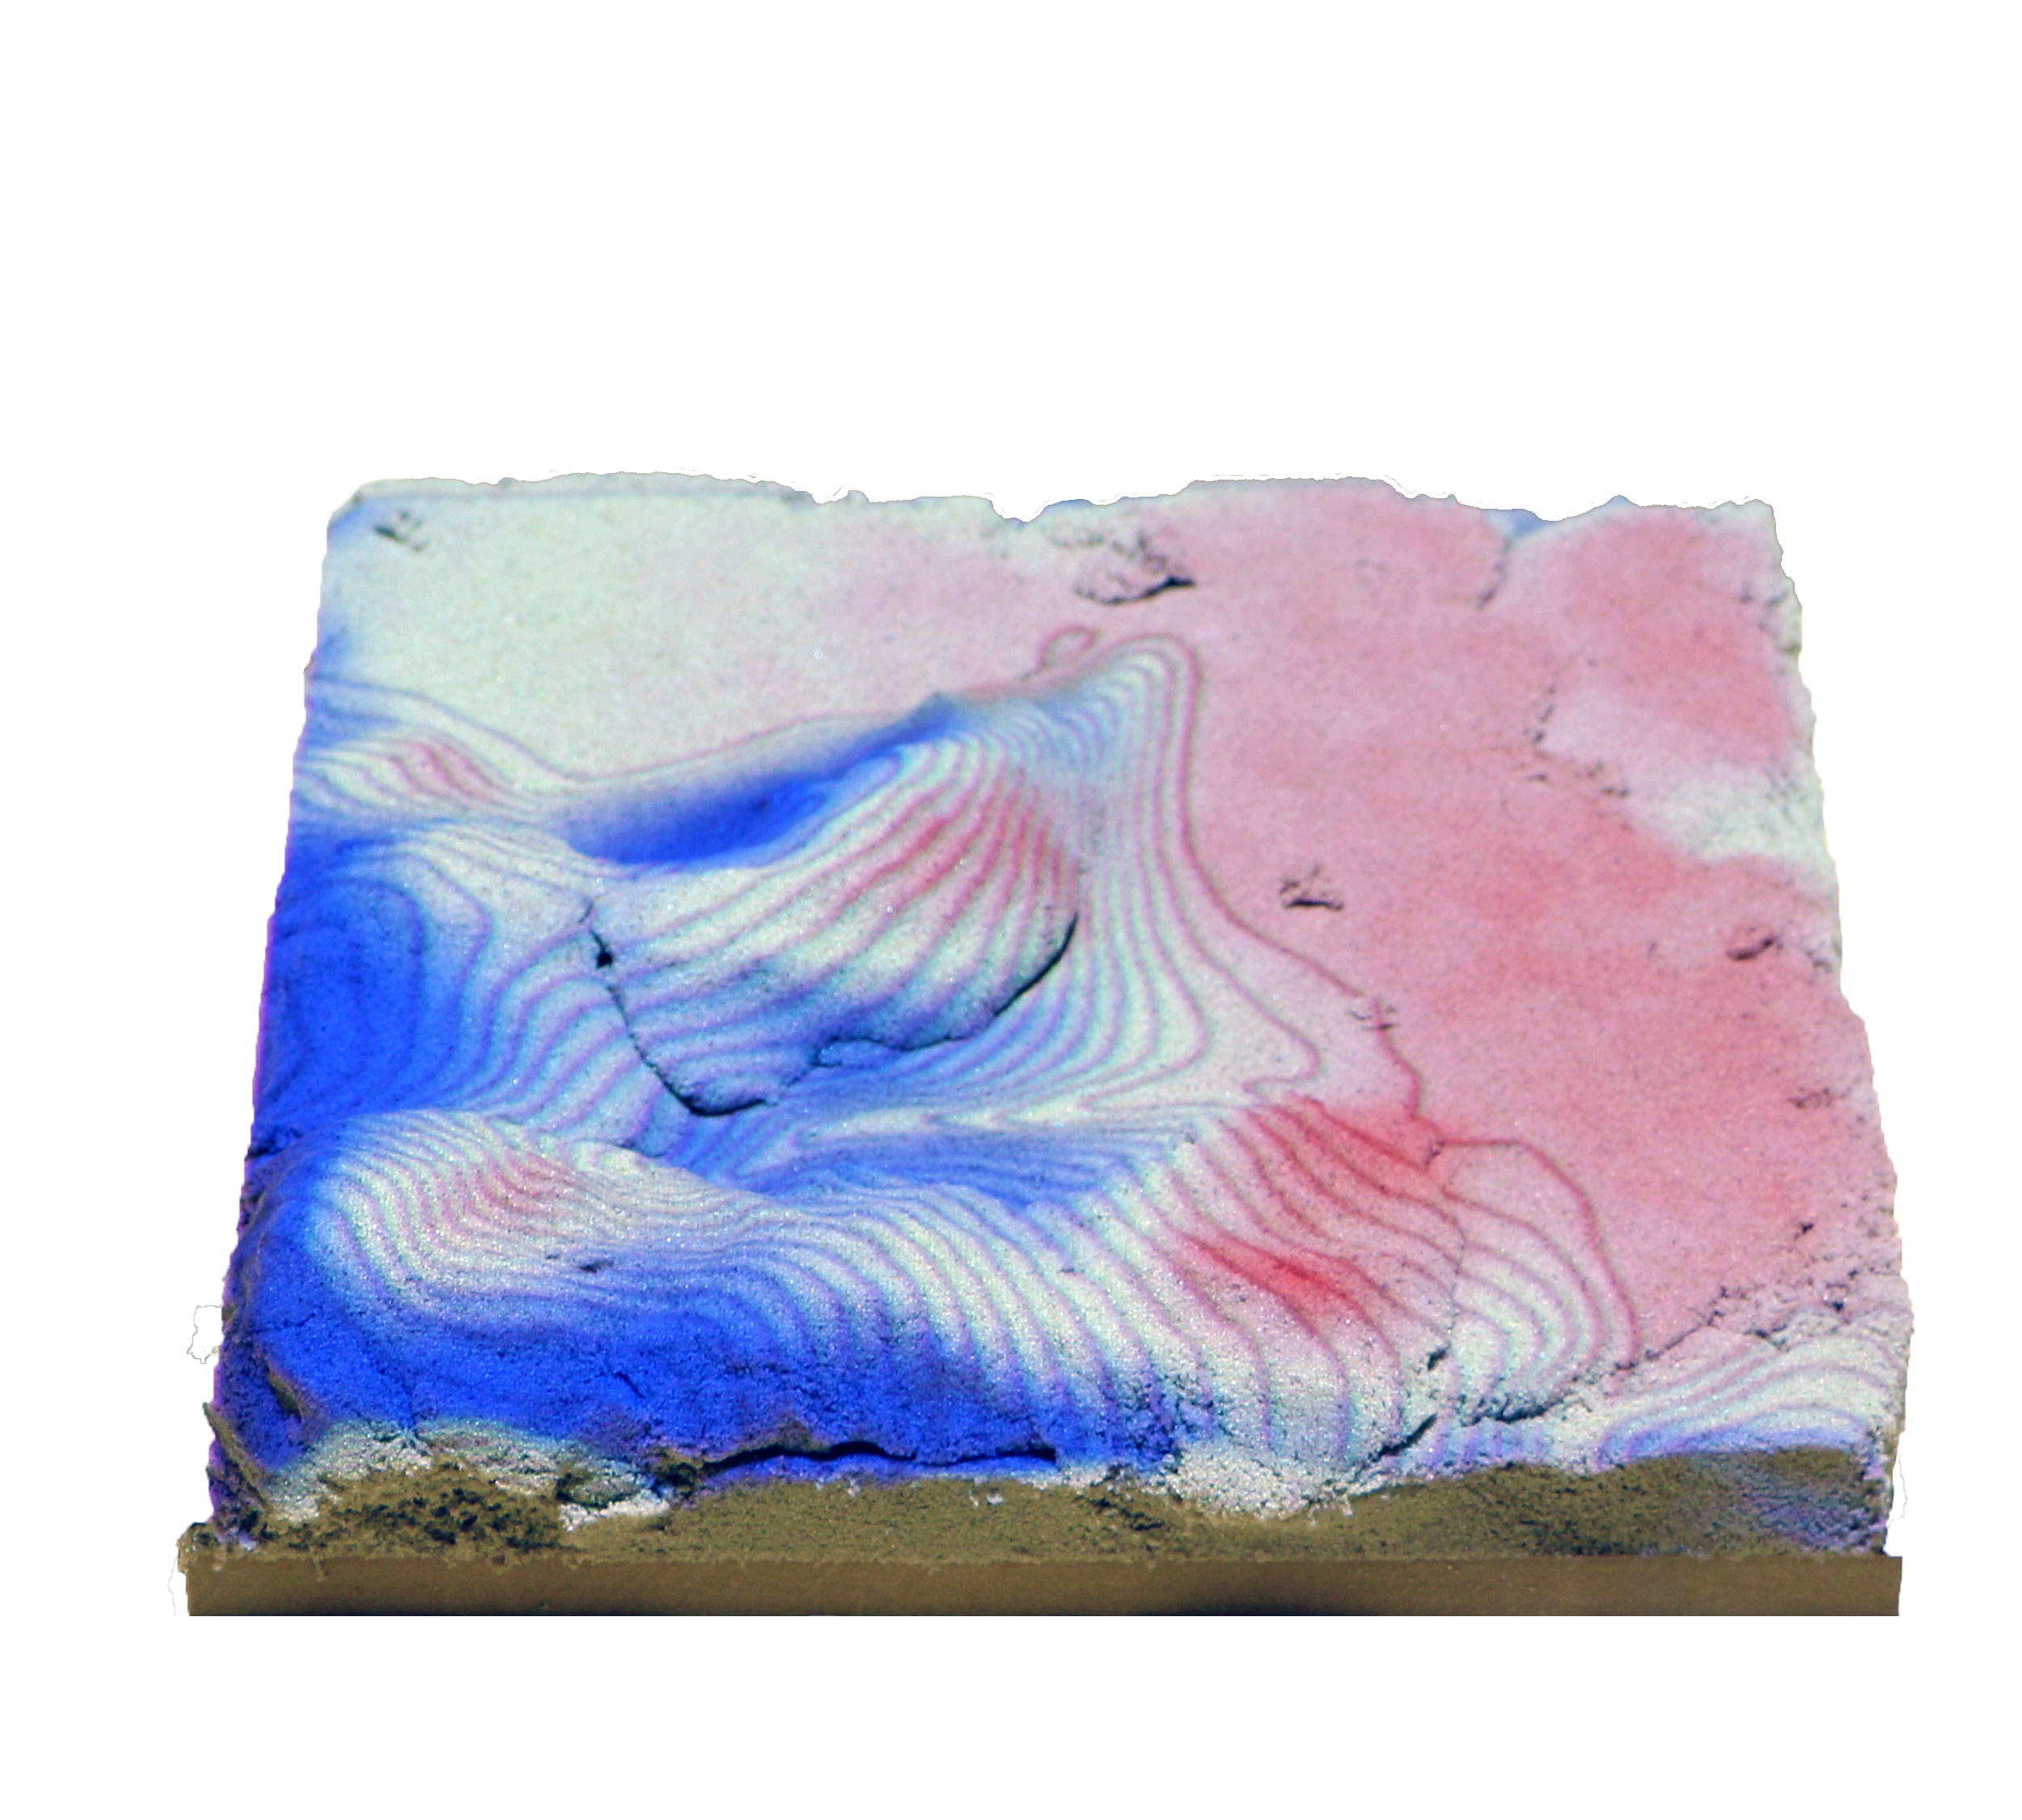
\includegraphics[width=\textwidth]{figures/tl/tl_difference_s_3.png}
                %\includegraphics[width=\textwidth]{images/art_diff_3}
                %\caption{Updated water flow}
                \caption{}
                \label{fig:sequence_0_4}
        \end{subfigure}
        ~ %add desired spacing between images, e. g. ~, \quad, \qquad, \hfill etc.
        \caption{3D sketching with Tangible Landscape: %
        (a) a cycle of scanning and projection couples a physical and digital model, %
        (b) the differencing analytic with blue where sand should be added and red where sand should be removed, %
        (c) a participant adding sand, and %
        (d) the updated differencing analytic. %
        }
        \label{fig:3d_sketching_1}
\end{figure*}
%
\setlength{\belowcaptionskip}{0em}

% experiment
I have conducted a rigorous experiment
using geospatial analytics to
compare spatial performance 
in analog modeling by hand,
in tangible computing using Tangible Landscape,
and in visual computing using 3D modeling programs via a GUI.
% tangible landscape
Tangible Landscape is a continuous shape display
tightly integrated with GRASS GIS 
that was designed to intuitively 3D sketch landscapes (Figure~\ref{fig:3d_sketching_1}).
Conceptually, Tangible Landscape couples 
a physical model with a digital model 
in a real-time feedback cycle of 
3D scanning, geospatial modeling and simulation, 
and projection (Figure~\ref{fig:schema}) \cite{Petrasova2015}. %Tateosian2010 %Petrasova2014

% methods
I have begun to test my hypotheses 
using quantitative methods %and qualitative methods.
%using qualitative methods 
%including semi-structured interviews and direct observation
%and quantitive methods including geospatial modeling, 
%analysis, simulation, and statistics.
Rather than studying basic spatial cognitive abilities that can not 
usefully be disentangled in applied use,
I am studying applied spatial cognitive processes 
using the metrics and parameters of the given application.
I am studying how participants perform 
in a series of time constrained terrain modeling 
exercises using analog modeling, visual computing, and tangible computing.
6 landscape architects and 6 geospatial analysts 
%ranging from novices to experts in their fields 
have participated in this pilot study. 
I am assessing their performance with each technology using 
spatial statistics, topographic parameters, morphology, 
process-form interactions, and differencing. 
%I use a fast, fluid, iterative process as a proxy for creative thinking 
%that can be assessed using these methods.
%qualitatively through interviews and observation and
%quantitatively through geospatial analyses and spatial statistics. 

\subsection{Terrain modeling experiment}
% landscape
%In each exercise participants are asked to model a different region 
%of a real landscape -- Lake Raleigh Woods 
%on North Carolina State University's Centennial Campus -- 
%from a flat surface using a different technology. 
%We use a real landscape because 
%computer generated landscapes look surreal and may lack distinct landforms. 
%We selected regions of the landscape that had distinctive, 
%clearly defined landforms so that participants would have different, 
%but analogous challenges for each exercise. 

% exercises
The \nth{1} exercise tests spatial performance in analog modeling 
to establish the baseline spatial ability of each participant.
In this exercise participants 
sculpt a given terrain in polymeric sand using their hands
with a CNC routed model for reference.
%(Figure~\ref{fig:exercise_1}).

The \nth{2} exercise tests spatial performance 
in projection augmented analog modeling 
to establish a baseline for spatial performance in tangible computing.
In this exercise participants 
sculpt a given terrain in polymeric sand 
using a projected map of the given elevation 
and contours as a guide.
%(Figure~\ref{fig:exercise_2}).

The \nth{3}-\nth{5} exercises test spatial performance 
in tangible computing augmented with different analytics.
In the \nth{3} exercise participants use Tangible Landscape to 
sculpt a given terrain in polymeric sand 
using the given and scanned contours as a guide. 
%(Figure~\ref{fig:exercise_3}).
In the \nth{4} exercise participants use Tangible Landscape to 
sculpt a given terrain in polymeric sand 
using the difference between the given 
and the scanned landscape as a guide. 
%(Figure~\ref{fig:exercise_4}).
In the \nth{5} exercise participants use Tangible Landscape to 
sculpt a given terrain in polymeric sand 
using the simulated water flow 
over the scanned landscape
as a guide 
in order to study 4D thinking.
% process-form interaction
%(Figure~\ref{fig:exercise_5}).

The \nth{6} and \nth{7} exercises test spatial performance in visual computing.
In the \nth{6} exercise 
participants digitally sculpt a given terrain in Rhinoceros, 
%a non-uniform rational B-spline (NURBS)-based 3D modeling program, 
a 3D modeling program, 
using the given 3D contours as a guide. 
%(Figure~\ref{fig:exercise_6}).
In the \nth{7} exercise 
participants digitally sculpt a given terrain in VUE,
%a triangulated irregular network (TIN)-based 
a 3D modeling program
designed for intuitive terrain sculpting, 
with a CNC routed model for reference. 
%(Figure~\ref{fig:exercise_7}).

\subsection{Data collection and analysis}
%\subsection{Quantitative data collection and analysis}
In the \nth{1}-\nth{5} exercises the resulting physical models are 3D scanned, 
imported into GRASS GIS as point clouds, and 
interpolated as DEMs for analysis. 
In the \nth{6} and \nth{7} exercises the resulting digital models are 
exported as point clouds, imported into GRASS GIS, 
and interpolated as DEMs for analysis. 
For each model I compute the elevation and its histogram 
and bivariate scatterplot, the slope, the difference and its histogram, 
the simulated water flow, and morphology. 
For each exercise I compute 
a map of the coefficient of variance of all the of DEMs,
bivariate scatterplots of
the covariance and correlation matrix of all the of DEMs,
and the mean and the absolute value of the mean of the 
differences between the the reference terrain and the modeled terrain.

%\subsection{Qualitative data collection and analysis}
%The design of the experiment was based on extensive case studies in 
%3D modeling, geospatial modeling, and tangible interaction 
%\cite{Tateosian2010, Petrasova2015}.  
%During the experiment the participants creative processes
%were observed and documented
%with photographs and notes. 
%Semi-structured interviews were conducted with select participants
%after the experiment. 
%The interviews were focused on 
%the intuitiveness and affordances of each technology, 
%strategies and modes of representation, 
%participants' understanding of space in a given medium,
%and their creative process.

\subsection{Code}
As a work of open science 
the data and the python scripts for data analysis are 
publicly available on GitHub at \url{https://github.com/baharmon/tangible_topography}
released under the GNU General Public License version 2. 
Both GRASS GIS and Tangible Landscape 
are open source projects
released under the GNU General Public License version 2. 
Tangible Landscape is available on GitHub at 
\url{https://github.com/ncsu-osgeorel/grass-tangible-landscape}.

%------------------------- RESULTS ---------------------------------------------

\section{Preliminary results}

%I have analyzed 12 of the participants' results as a pilot study. 
Select results for one participant in the pilot study are shown in 
Figures~\ref{fig:reference},~\ref{fig:results_2},~and~\ref{fig:results_6}.

In the \nth{1} exercise participants tended to model the overall form well, 
but exaggerated the slopes and misplaced the main ridge. 
%
In the \nth{2} exercise participants tended to model the landscape very well, 
accurately capturing the ridge and valley, but missing the saddle of the valley 
(Figure \ref{fig:diff_stddev_2}).
%
In the \nth{3} exercise participants tended to model the overall form well, but 
approximately with indistinct landforms and a lot of roughness. 
Many participants used a layered \emph{pancake}-modeling strategy here.
%
The \nth{4} exercise tended to have the best results. 
Participants used a rapid iterative process 
to accurately model the landscape. 
%Most were too busy refining the form
%to smooth their models
%and thus had rough microtopography.
%
In the \nth{5} exercise participants tended to model the overall form well, but 
exaggerated the slopes of the stream channels. 
%
In the \nth{6} exercise most participants modeled the form very poorly
especially the interior space
(Figure \ref{fig:diff_stddev_6})  
-- either modeling only the edges or 
modeling very approximate massings of 
the main ridge and peak. 
Expert 3D modelers, however, modeled the form better, 
but still missed much of the interior space.
%
In the \nth{7} exercise participants tended to model 
the landscape suggestively in the x- and y-dimensions,
but underestimated and grossly distorted the z-dimension. 
%with correct, yet exaggerated and rough landforms.
%They, however, tended to grossly distort the z-dimension. 

The pilot study suggests that  
\begin{enumerate*}[label=\bfseries \arabic*.]
\item %
analog sculpting by hand can be highly intuitive, 
but the lack of analytical feedback limits 
ones ability to critique the model and refine its form,
\item %
shape displays like Tangible Landscape can be intuitive, 
enhance spatial performance,
and enable rapid iteration and thus creative spatial learning.
\item %
digital sculpting via a graphical user interface 
is unintuitive and visually ambiguous 
leading to misinterpretations of depth, height, and interior space.
\end{enumerate*} 

%
\setlength{\belowcaptionskip}{-1em}
%
\begin{figure}[h]
        \centering
        \begin{subfigure}[t]{0.225\textwidth}
                \includegraphics[width=\textwidth]{figures/series/diff_stddev_2.png}
                %\caption{Ex.~2: projection augmented}
                \caption{}~\label{fig:diff_stddev_2}
        \end{subfigure}
        ~ %add desired spacing between images, e. g. ~, \quad, \qquad, \hfill etc.
        \begin{subfigure}[t]{0.225\textwidth}
                \includegraphics[width=\textwidth]{figures/series/diff_stddev_6.png}
                %\caption{Ex.~6: Rhinoceros}
                \caption{}~\label{fig:diff_stddev_6}
        \end{subfigure}
        ~ %add desired spacing between images, e. g. ~, \quad, \qquad, \hfill etc.
        \caption{Standard deviations of the differences for all participants: %
        (a) in Ex.~2 using projection augmented modeling and %
        (b) in Ex.~6 using Rhinoceros. %        
        }
        \label{fig:diff_stddev}
\end{figure}
%
\setlength{\belowcaptionskip}{0em}
%

%------------------------- FIGURE ---------------------------------------------

\begin{figure*}
%
    \begin{minipage}[t]{0.33\textwidth}
        %
        \begin{subfigure}{\linewidth}
            \centering
            \includegraphics[width=\textwidth]{figures/reference/dem_1.png}%
            \caption{}~\label{fig:ref}
        \end{subfigure}\\
        %
        \begin{subfigure}{\linewidth}
            \centering
            \includegraphics[width=\textwidth]{figures/reference/diff_1.png}%
            \caption{}~\label{fig:diff}
        \end{subfigure}\\
        %
        \begin{subfigure}{\linewidth}
            \centering
            \includegraphics[width=\textwidth]{figures/reference/bivariate_1.png}%
            \caption{}~\label{fig:bivar}
        \end{subfigure}\\
        \vspace{1.25em}
        %
        \captionsetup{width=.9\linewidth}
        \caption{\textbf{Reference model:} \\
        (a) the digital elevation model (DEM), \\
        (b) the difference between the reference DEM and the reference DEM, and \\
        (c) the bivariate scatterplot of the difference between the reference DEM and the reference DEM. %
        }~\label{fig:reference}
        %
    \end{minipage}
%
    \begin{minipage}[t]{0.33\textwidth}
        %
        \begin{subfigure}{\linewidth}
            \centering
            \includegraphics[width=\textwidth]{figures/magallanes/magallanes_dem_2.png}%
            \caption{}~\label{fig:dem_2}
        \end{subfigure}\\
        %
        \begin{subfigure}{\linewidth}
            \centering
            \includegraphics[width=\textwidth]{figures/magallanes/magallanes_diff_2.png}%
            \caption{}~\label{fig:diff_2}
        \end{subfigure}\\
        %
        \begin{subfigure}{\linewidth}
            \centering
            \includegraphics[width=\textwidth]{figures/magallanes/magallanes_bivariate_2.png}%
            \caption{}~\label{fig:bivar_2}
        \end{subfigure}\\ 
        %
        \captionsetup{width=.9\linewidth}
        \caption{\textbf{Participant's model for Ex.~2 using projection augmented modeling:} \\
        (a) the DEM, \\
        (b) the difference between the participant's DEM and the reference DEM, and \\
        (c) the bivariate scatterplot of the difference between the participant's DEM and the reference DEM. %
        }~\label{fig:results_2}
        %
    \end{minipage}
%
    \begin{minipage}[t]{0.33\textwidth}
        %
        \begin{subfigure}{\linewidth}
            \centering
            \includegraphics[width=\textwidth]{figures/magallanes/magallanes_dem_6.png}%
            \caption{}~\label{fig:dem_6}
        \end{subfigure}\\
        %
        \begin{subfigure}{\linewidth}
            \centering
            \includegraphics[width=\textwidth]{figures/magallanes/magallanes_diff_6.png}%
            \caption{}~\label{fig:diff_6}
        \end{subfigure}\\
        %
        \begin{subfigure}{\linewidth}
            \centering
            \includegraphics[width=\textwidth]{figures/magallanes/magallanes_bivariate_6.png}%
            \caption{}~\label{fig:bivar_2}
        \end{subfigure}\\
        %
        \captionsetup{width=.9\linewidth}
        \caption{\textbf{Participant's model for Ex.~6 using digital sculpting with Rhinoceros:} \\
        (a) the DEM, \\
        (b) the difference between the participant's DEM and reference DEM, and \\
        (c) the bivariate scatterplot of the difference between the participant's DEM and the reference DEM. %
        }~\label{fig:results_6}
        %
    \end{minipage}
%
\end{figure*}
%

%------------------------- FUTURE WORK ---------------------------------------------

% An outline of the activities done so far and activities planned 
% for the remainder of the PhD. 

\section{Future work}
The full study will have approximately 40 participants. 
Based on the results of the study
I hope to develop a theory 
of how technology mediates spatial cognition.
% 
In the long-term I plan to expand this study of 
embodied spatial cognition in tangible computing
as a collaborative research project with psychologists
using spatial analytics, eye tracking, biometric sensors, and EEGs.
%electroencephalograms

%I will analyze all of the participants' results, interpret the data, 
%test my hypotheses, develop a theory 
%of how technology mediates spatial cognition and creativity,
%and publish the completed research. 
%I will also continue designing and contributing 
%to Tangible Landscape. 

%Once I finish this study
%I intend to submit and defend my dissertation
%by the end of this academic year. 

%------------------------- CONCLUSION ---------------------------------------------

\section{Conclusions}

% unique contribution: geospatial analysis of tangible interaction
This study is unique in applying geospatial analyses 
to asses spatial performance in tangible interaction.
% brief summary of findings 
My initial findings suggest that 
shape displays like Tangible Landscape can 
with the right computational analytics
enhance performance in novel ways
and enable rapid iterations of generative form-finding and critical analysis.
Different analytics encourage 
significantly different modes of spatial thinking 
and strategies for modeling. 
The differencing analytic leads to significant improvements 
in spatial performance and enables an iterative process. 

% implications for design




%It is important that you write for the SIGCHI audience. Please read
%previous years' proceedings to understand the writing style and
%conventions that successful authors have used. It is particularly
%important that you state clearly what you have done, not merely what
%you plan to do, and explain how your work is different from previously
%published work, i.e., the unique contribution that your work makes to
%the field. Please consider what the reader will learn from your
%submission, and how they will find your work useful. If you write with
%these questions in mind, your work is more likely to be successful,
%both in being accepted into the conference, and in influencing the
%work of our field.

%------------------------- ACKNOWLEDGEMENTS ----------------------------------

\section{Acknowledgments}
My colleagues 
in the NCSU Open Source Geospatial Research and Education Lab
(\url{http://geospatial.ncsu.edu/osgeorel/})
Anna Petrasova, Vaclav Petras, Helena Mitasova, and Ross Meentemeyer 
contributed to this research by
collaboratively designing Tangible Landscape and 
helping to run the experiment.

%------------------------- FIGURES ---------------------------------------------
%The paper may be accompanied by a short video figure up to five
%minutes in length. However, the paper should stand on its own without
%the video figure, as the video may not be available to everyone who
%reads the paper.  

%References should be in ACM citation format:
%\url{http://www.acm.org/publications/submissions/latex_style}.  
%DOI and/or URL links are
%optional but encouraged as are full first names. Note that the
%Hyperlink style used throughout this document uses blue links;
%however, URLs in the references section may optionally appear in
%black.
%For papers from
%conference proceedings, include the title of the paper and the name of
%the conference. Do not include the location of the conference or the
%exact date; do include the page numbers if available. 

%------------------------- REFERENCES ---------------------------------------------

%\balance{}
\bibliographystyle{SIGCHI-Reference-Format}
\bibliography{tangible_topography.bib}

%------------------------- END ---------------------------------------------

\end{document}

%%% Local Variables:
%%% mode: latex
%%% TeX-master: t
%%% End:
